\section{Complexity of Arithmetic Operations}

We want to talk about basic operations (i.e. $\{+, -, \times, \div \}$) over a \underline{ring}. (Note: Division may not always be possible)

\begin{example}{Rings}{}
    The following rings will come up:
    \begin{enumerate}
        \item Integers ($\Z$)
        \item Rationals ($\Q$)
        \item Fields (E.g. $\Z_7$)
        \item Polynomial Rings ($R[x]$), where $R$ is any commutative ring. E.g. $\Z[x], \Q[x], \Z_p[x]$
        \item Field of rational functions ($R(x)$). E.g. $\Q(x)$
    \end{enumerate}
\end{example}

\subsection{Naïve upper bounds on costs}
For polynomials, we are interested in $a,b \in R[x]$. We will let $n = deg(a),\ m = deg(b)$ and we will count ring operations from $R$.

For integers, we will count bit operations.

We'll also define the following operation: for $a \in \Z$, $\lg a = \begin{cases}1 \quad \text{if } a = 0 \\ 1 + \left \lfloor \log_2 |a| \right\rfloor \quad \text{if } a \neq 0 \end{cases}$

The following table summarizes the upper bounds:
\begin{center}
\begin{tabular}{c|c|c}
    Operation & Polynomials & Integers \\
    \hline
    $a + b$ & $n + m + 1$ & $\lg a + \lg b$\\
    $a - b$ & $n + m + 1$ & $\lg a + \lg b$\\
    $a \times b$ & $(n+1)(m+1)$ & $(\lg a)(\lg b)$\\
    $a = qb + r$ & $(n-m+1)(m+1)$ & $(\lg \frac{a}{b})(\lg b)$
\end{tabular}
\end{center}

\subsubsection{Addition}

\begin{center}
\begin{tabular}{ll}
    $a_0 + a_1x + \ldots + a_mx^m +$ & $a_{m+1}x^{m+1} + \ldots + a_nx^n$ \\
    $b_0 + b_1x + \ldots + b_mx^m$ & \\
    \hline
    $c_0 + c_1x + \ldots + c_mx^m +$ & $c_{m+1}x^{m+1} + \ldots + c_nx^n$ \\
\end{tabular}
\end{center}

While we really only add the first $m+1$ terms, the add operation returns a new polynomial $c$.
As such, we really perform $\max\{m,n\} + 1 \in \Theta(n + m) + 1$ operations.

The same analysis can be used for the add operation on integers. 

\subsubsection{Multiplication}

Consider $a = \sum^n a_i x^i, b = \sum^m b_i x^i$, and $c = a \times b = \sum^{n + m} c_k x^k$, where $c_k = \sum a_i b_j$.

Classical ``school'' method: Cost is $(n + 1)(m + 1)$ multiplications and $nm$ additions (exactly).

\subsubsection{Division with Remainder}
Given $a,b \in \Z$ (or $R[x]$), we want to find $q, r \in \Z$ with $size(r) < size(b)$ so that $a = bq + r$. Note that: $size(\cdot)$ for integers is just the magnitude, and for polynomials, $size(r) = \deg(r)$

We will require that for polynomials $a,b$, in $a \div b$, the constant term of $b$ is a unit (and so an inverse exists)

Doing long division results in something that will look like the drawing below:
\begin{figure}[h]
    \centering
    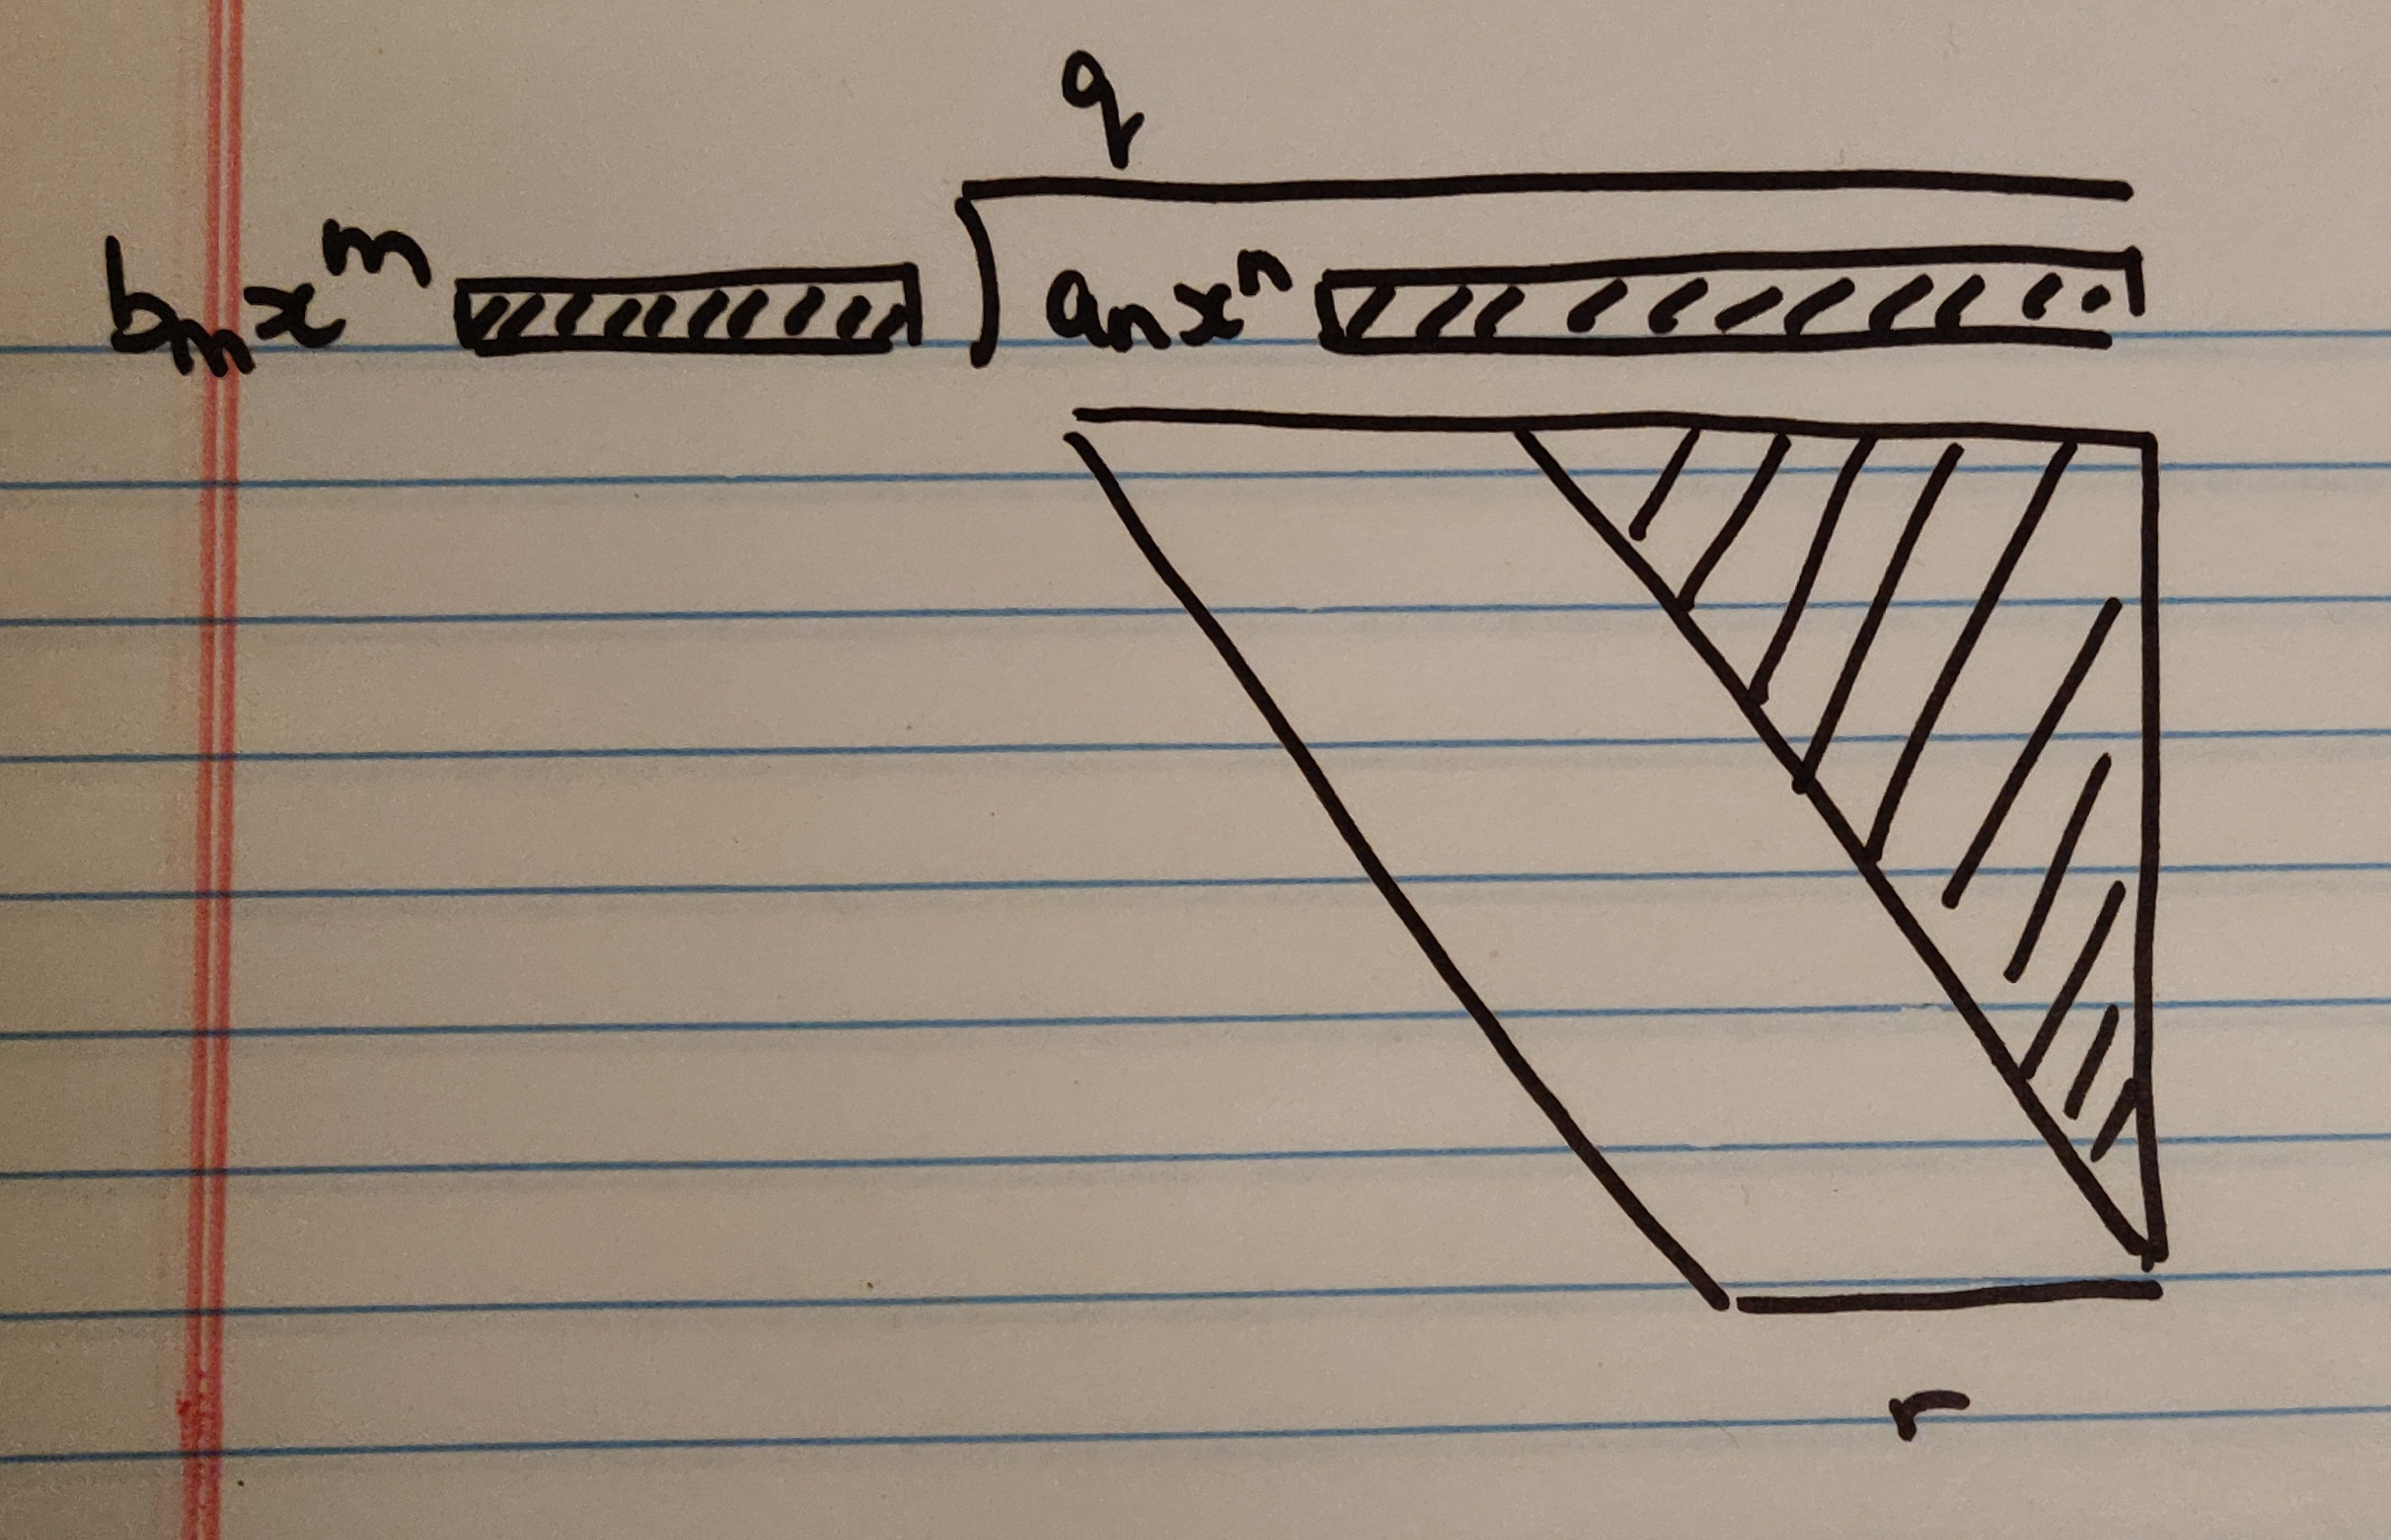
\includegraphics[width=0.6\textwidth]{images/lec2-long-division}
\end{figure}

Within the shaded region of the trapezoid, no changes are made to the polynomial.
In each step of the long division, we only perform changes to $m$ terms within the unshaded band in the trapezoid.
There are a total of $n-m$ steps (This is the resulting degree of $q$).

So, in total, long division of polynomials can be done in $\\bigO{O}((m+1)(n-m+1))$ operations.

\begin{note}
    Why do we not just reuse our subtraction operation? We want this division operation to be primitive. The operation only performs ring operations as needed.
\end{note}

The same analysis can be performed on long division of integers.

\subsection{Multimodular Reduction}
Suppose $a \in \Z$, $p_1, \ldots, p_k \in \Z_{> 1}$, with $a < p := p_1\ldots p_k$. What is cost of computing $a \mod p_1$, $a \mod p_2$, $\ldots$, $a \mod p_k$? (i.e. Obtaining the remainders)

\underline{Rough Bound:} We can use the division with remainder operation.
Both $a$ and the $p_i$'s are bounded by $p$.
Since there are $k$ $p_i$'s, we will perform the operation at most $k$ times.
This gives the bound $\bigO(k(\lg p)^2)$

But, of course we can be more accurate with this bound.
In total, the $k$ division with remainders require $\sum_{i = 1}^k C\left(\lg \frac{a}{p_i}\right)\left(\lg p\right)$ operations (The $C$ comes from the big-$\bigO$ of the division with remainder operation).
We get:
\begin{equation*}
\begin{aligned}
    &\sum_{i = 1}^k C\left(\lg \frac{a}{p_i}\right)\left(\lg p\right)\\
    &= C \sum_{i = 1}^k \left(\lg \frac{a}{p_i}\right)\left(\lg p\right) \\
    &\leq C \left(\lg p\right) \sum_{i = 1}^k \left(\lg p\right) \quad &(\lg \frac{a}{p_i} \leq \lg a \leq \lg p) \\
    &\leq C (1 + \log p) \sum_{i = 1}^k (1 + \log p) \quad & (\text{Get rid of the }\lg)\\
    &\leq C (2\log p) \sum_{i = 1}^k (2\log p) \quad & (\text{If } x > 1, 1 + \log x \leq 2\log x)\\
    &=4C(\log p)^2
\end{aligned}
\end{equation*}